\subsection{Exercises}
\label{ch:11ex}


%%%%%%%%%%%%%%%%%%%%%%%%%%%%%%
\Large{Problem 11.1}
\begin{figure}[H]
    \centering
    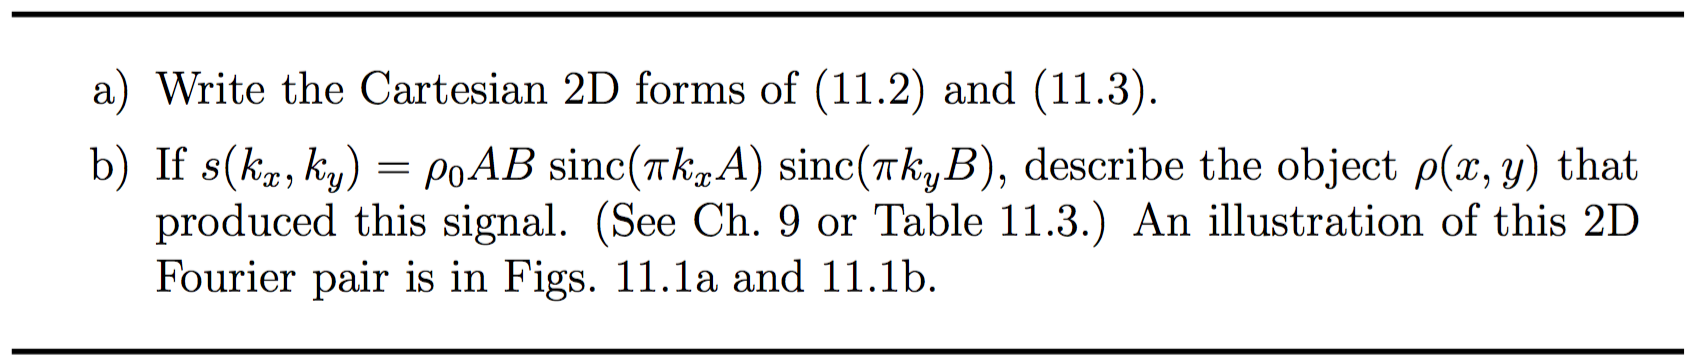
\includegraphics[width=1\textwidth,keepaspectratio]{prbl111}
    \label{fig:prbl111}
\end{figure}

%%%
\textit{Remember:}
\begin{itemize}
	\item We used: $rect(\frac{x}{W}) \xLeftrightarrow{\mathfrak{F}} W sinc(\pi W k)$
\end{itemize}


%%%
\textit{Definitions:}
\begin{flalign*}
    H(k) \equiv \mathfrak{F}(h(x)) & = \int_{- \infty}^{\infty} dx \  h(x) e^{- i 2 \pi k x} \\
    h(x) \equiv \mathfrak{F}^{-1}(H(k)) & = \int_{- \infty}^{\infty} dk \ H(k) e^{+ i 2 \pi k x}
\end{flalign*}

%%%
\textit{a) Proof.}
\begin{flalign*}
    H(k_x, k_y) \equiv \mathfrak{F}(h(x, y)) & = \int_{- \infty}^{\infty} \int_{- \infty}^{\infty} dx dy \  h(x,y) e^{- i 2 \pi (k_x x + k_y y)} \\
    h(x, y) \equiv \mathfrak{F}^{-1}(H(k_x, k_y)) & = \int_{- \infty}^{\infty} \int_{- \infty}^{\infty} dk_x dk_y \ H(k_x, k_y) e^{+ i 2 \pi (k_x x + k_y y)}
\end{flalign*}

%%%
\textit{b) Proof.}
\begin{flalign*}
    \rho(x, y) & \equiv \mathfrak{F}^{-1}(s(k_x, k_y)) = \\
    & = \int_{- \infty}^{\infty} \int_{- \infty}^{\infty} dk_x dk_y \ s(k_x, k_y) e^{+ i 2 \pi (k_x x + k_y y)} \\
    & = \int_{- \infty}^{\infty} \int_{- \infty}^{\infty} dk_x dk_y \ \rho_0 AB sinc(\pi k_x A) \ sinc(\pi k_y B) e^{+ i 2 \pi (k_x x + k_y y)} \\
    & = \rho_0 \int_{- \infty}^{\infty} dk_x \ A sinc(\pi k_x A) \ e^{+ i 2 \pi k_x x} \int_{- \infty}^{\infty} dk_y \ B sinc(\pi k_y B) \ e^{+ i 2 \pi k_y y}\\
    & = \rho_0  \ \mathfrak{F}(B sinc(\pi k_y B)) \int_{- \infty}^{\infty} dk_x \ A sinc(\pi k_x A) \\
    & = \rho_0 \ \mathfrak{F}(A sinc(\pi k_x A))  \ \mathfrak{F}(B sinc(\pi k_y B)) \\
    & = \rho_0 \ rect(\frac{x}{A}) \ rect(\frac{y}{B}) 
\end{flalign*}

\begin{figure}[H]
    \centering
    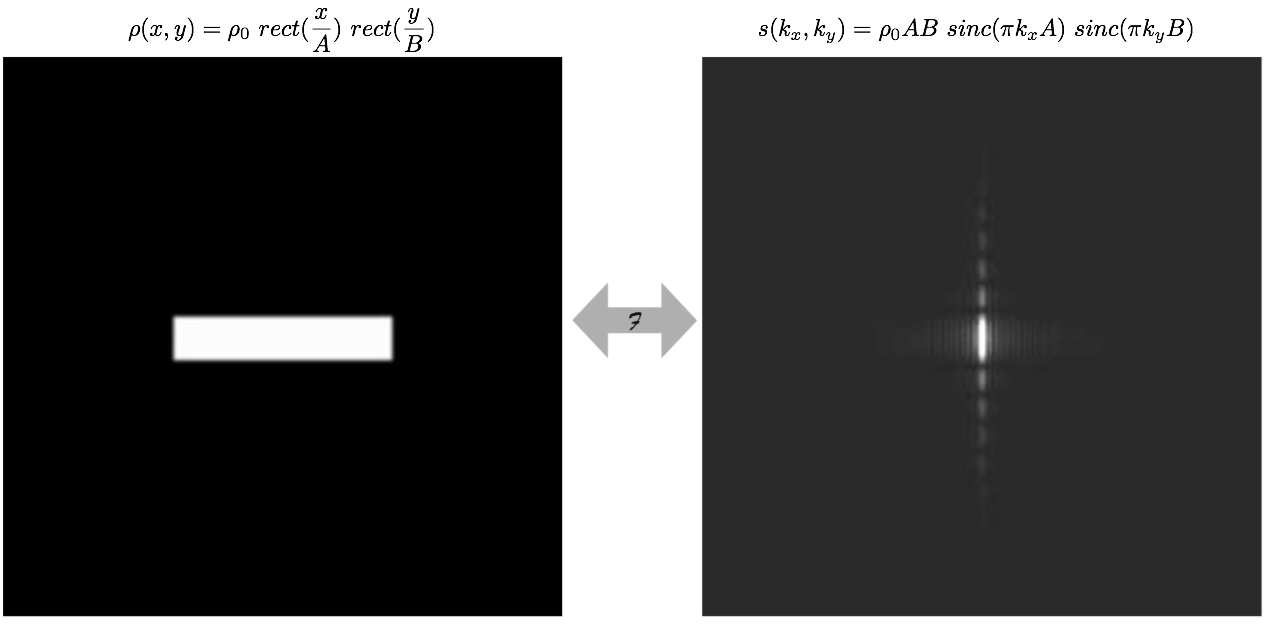
\includegraphics[width=1\textwidth,keepaspectratio]{prbl111i1}
    \label{fig:prbl111i1}
\end{figure}

\clearpage
%%%%%%%%%%%%%%%%%%%%%%%%%%%%%%

%%%%%%%%%%%%%%%%%%%%%%%%%%%%%%
\Large{Problem 11.2}
\begin{figure}[H]
    \centering
    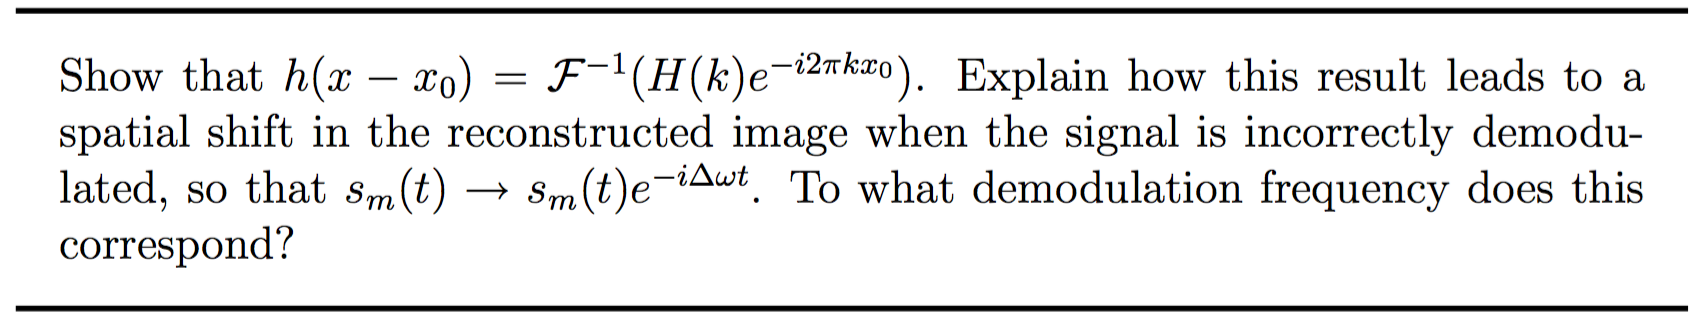
\includegraphics[width=1\textwidth,keepaspectratio]{prbl112}
    \label{fig:prbl112}
\end{figure}

%%%
\textit{Remember:}
\begin{itemize}
	\item The shift theorem:
    \begin{flalign*}
        \mathfrak{F}(h(x-x_0)) & = H(k) e^{-i 2 \pi k x_0} \\
        h(x-x_0) & = e^{-i 2 \pi k x_0} \mathfrak{F}^{-1}(H(k))
    \end{flalign*}          
\end{itemize}

%%%
\textit{Definitions:}
\begin{flalign*}
    H(k) \equiv \mathfrak{F}(h(x)) & = \int_{- \infty}^{\infty} dx \  h(x) e^{- i 2 \pi k x} \\
    h(x) \equiv \mathfrak{F}^{-1}(H(k)) & = \int_{- \infty}^{\infty} dk \ H(k) e^{+ i 2 \pi k x}
\end{flalign*}

%%%
\textit{Proof.}
\begin{flalign*}
    \text{Let } h(x') & = \mathfrak{F}^{-1}(H(k)) \Rightarrow \\
    h(x') & = \int_{- \infty}^{+ \infty} dk \ H(k) e^{+ i 2 \pi k x'} \\
    \text{Change of variable: } x' & = x - x_0 \Rightarrow \\
    h(x - x_0) & = \int_{- \infty}^{+ \infty} dk \ H(k) e^{+ i 2 \pi k (x-x_0)} \\
    & =\int_{- \infty}^{+ \infty} dk \ H(k)  e^{- i 2 \pi k x_0} \  e^{+ i 2 \pi k x} \\
    & = \mathfrak{F}^{-1}(H(k) \ e^{- i 2 \pi k x_0} )  
\end{flalign*}




\clearpage
%%%%%%%%%%%%%%%%%%%%%%%%%%%%%%

%%%%%%%%%%%%%%%%%%%%%%%%%%%%%%
\Large{Problem 11.3}
\begin{figure}[H]
    \centering
    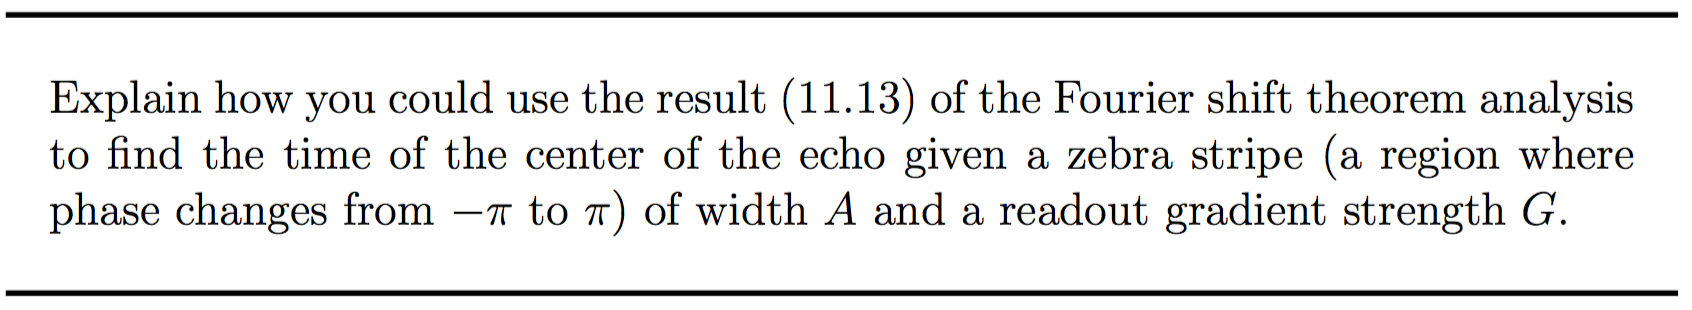
\includegraphics[width=1\textwidth,keepaspectratio]{prbl113}
    \label{fig:prbl113}
\end{figure}

\textit{Remember:}
\begin{itemize}
	\item 
\end{itemize}

\textit{Definitions:}


\textit{Proof.}

\clearpage
%%%%%%%%%%%%%%%%%%%%%%%%%%%%%%

%%%%%%%%%%%%%%%%%%%%%%%%%%%%%%
\Large{Problem 11.4} 

\begin{figure}[H]
    \centering
    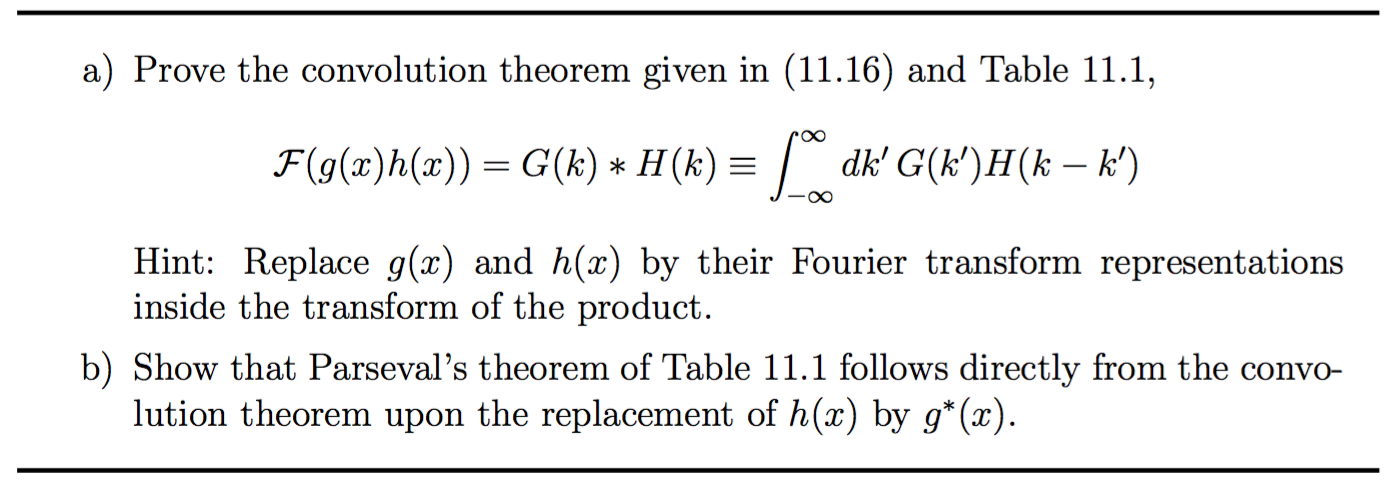
\includegraphics[width=1\textwidth,keepaspectratio]{prbl114}
    \label{fig:prbl114}
\end{figure}

\textit{Remember:}
\begin{itemize}
	\item 
\end{itemize}

\textit{Definitions:}
\begin{flalign*}
    H(k) \equiv \mathfrak{F}(h(x)) & = \int_{- \infty}^{\infty} dx \  h(x) e^{- i 2 \pi k x} \\
    h(x) \equiv \mathfrak{F}^{-1}(H(k)) & = \int_{- \infty}^{\infty} dk \ H(k) e^{+ i 2 \pi k x}
\end{flalign*}


\textit{a) Proof.} \label{proof:convolution}
\begin{flalign*}
\mathfrak{F}(g(x) h(x)) &= \int_{- \infty}^{\infty} dx \  g(x) h(x) e^{- i 2 \pi k x} \\
    &= \int_{- \infty}^{\infty} dx \  e^{- i 2 \pi k x} \  \int_{- \infty}^{\infty} dk' \ G(k') e^{+ i 2 \pi k' x} \  \int_{- \infty}^{\infty} dk'' \ H(k'') e^{+ i 2 \pi k'' x} \\
    &= \int_{- \infty}^{\infty} dx \  e^{- i 2 \pi k x} \  \int_{- \infty}^{\infty} dk' \ G(k') \  \int_{- \infty}^{\infty} dk'' \ H(k'') e^{+ i 2 \pi (k'+k'') x} \\
    & \text{Change of variable: } k' + k'' = k'''  \rightarrow k'' = k''' - k' \\
    &= \int_{- \infty}^{\infty} dx \  e^{- i 2 \pi k x} \  \int_{- \infty}^{\infty} dk' \ G(k') \  \int_{- \infty}^{\infty} dk''' \ H(k'''-k') e^{+ i 2 \pi k''' x} \\
    &= \int_{- \infty}^{\infty} dx \  e^{- i 2 \pi k x} \  \int_{- \infty}^{\infty} dk''' \ e^{+ i 2 \pi k''' x} \  \int_{- \infty}^{\infty} dk' \ G(k') H(k'''-k')  \\
    & \text{Notation: } W(k''') = \int_{- \infty}^{\infty} dk' \ G(k') H(k'''-k') \\
    &= \int_{- \infty}^{\infty} dx \  e^{- i 2 \pi k x} \  \int_{- \infty}^{\infty} dk''' \  W(k''') e^{+ i 2 \pi k''' x} \\
    &= \int_{- \infty}^{\infty} dx \  w(x) e^{- i 2 \pi k x} \\
    &= W(k) \\
    &= \int_{- \infty}^{\infty} dk' \ G(k') H(k-k') \equiv G(k) \ast H(k)
\end{flalign*}

\clearpage
\textit{b) Proof.} \label{proof:parseval}

\begin{flalign*}
\text{Let } g(x) = \int_{- \infty}^{\infty} dk' \ G(k') e^{+ i 2 \pi k' x} \text{ and } g^*(x) = \int_{- \infty}^{\infty} dk \ G^*(k'') e^{- i 2 \pi k'' x} \text{ then:}
\end{flalign*}

\begin{flalign*}
\int_{- \infty}^{+ \infty} dx \ \lvert g(x) \rvert ^2 &= \int_{- \infty}^{+ \infty} dx \ g(x) g^*(x) \\
    &= \int_{- \infty}^{+ \infty} dx \int_{- \infty}^{\infty} dk' \ G(k') e^{+ i 2 \pi k' x} \int_{- \infty}^{\infty} dk'' \ G^*(k'') e^{- i 2 \pi k'' x} \\
    &= \int_{- \infty}^{\infty} dk' \ G(k') \int_{- \infty}^{\infty} dk'' \ G^*(k'') \int_{- \infty}^{+ \infty} dx \ e^{- i 2 \pi (k''-k') x} \\
    & \text{We know that: } \delta(k-k_0) = \int_{- \infty}^{+ \infty} dx \ e^{- i 2 \pi (k-k_0) x} \Rightarrow \\
    &= \int_{- \infty}^{\infty} dk' \ G(k') \int_{- \infty}^{\infty} dk'' \ G^*(k'') \  \delta(k''-k') \\
    &= \int_{- \infty}^{\infty} dk' \ G(k') \ G^*(k') \\
    & \text{Substitute } k = k' \\
    &= \int_{- \infty}^{\infty} dk \ G(k) \ G^*(k) = \int_{- \infty}^{\infty} dk \ \lvert G(k)  \rvert ^2
\end{flalign*}

\clearpage
%%%%%%%%%%%%%%%%%%%%%%%%%%%%%%


%%%%%%%%%%%%%%%%%%%%%%%%%%%%%%
\Large{Problem 11.5}
\begin{figure}[H]
    \centering
    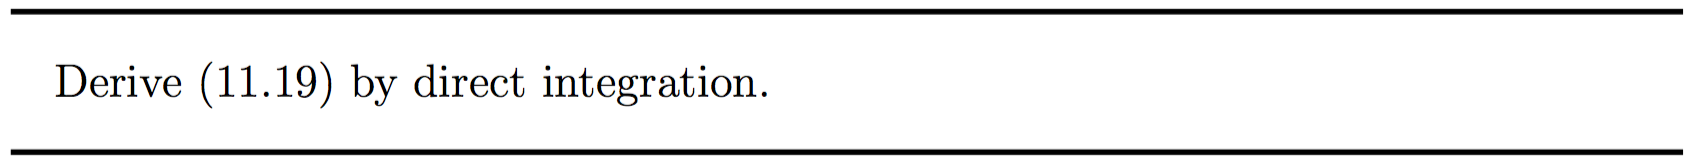
\includegraphics[width=1\textwidth,keepaspectratio]{prbl115}
    \label{fig:prbl115}
\end{figure}

\textit{Remember:}
\begin{itemize}
	\item 
\end{itemize}

\textit{Definitions:}


\textit{Proof.}

\clearpage
%%%%%%%%%%%%%%%%%%%%%%%%%%%%%%

%%%%%%%%%%%%%%%%%%%%%%%%%%%%%%
\Large{Problem 11.6}
\begin{figure}[H]
    \centering
    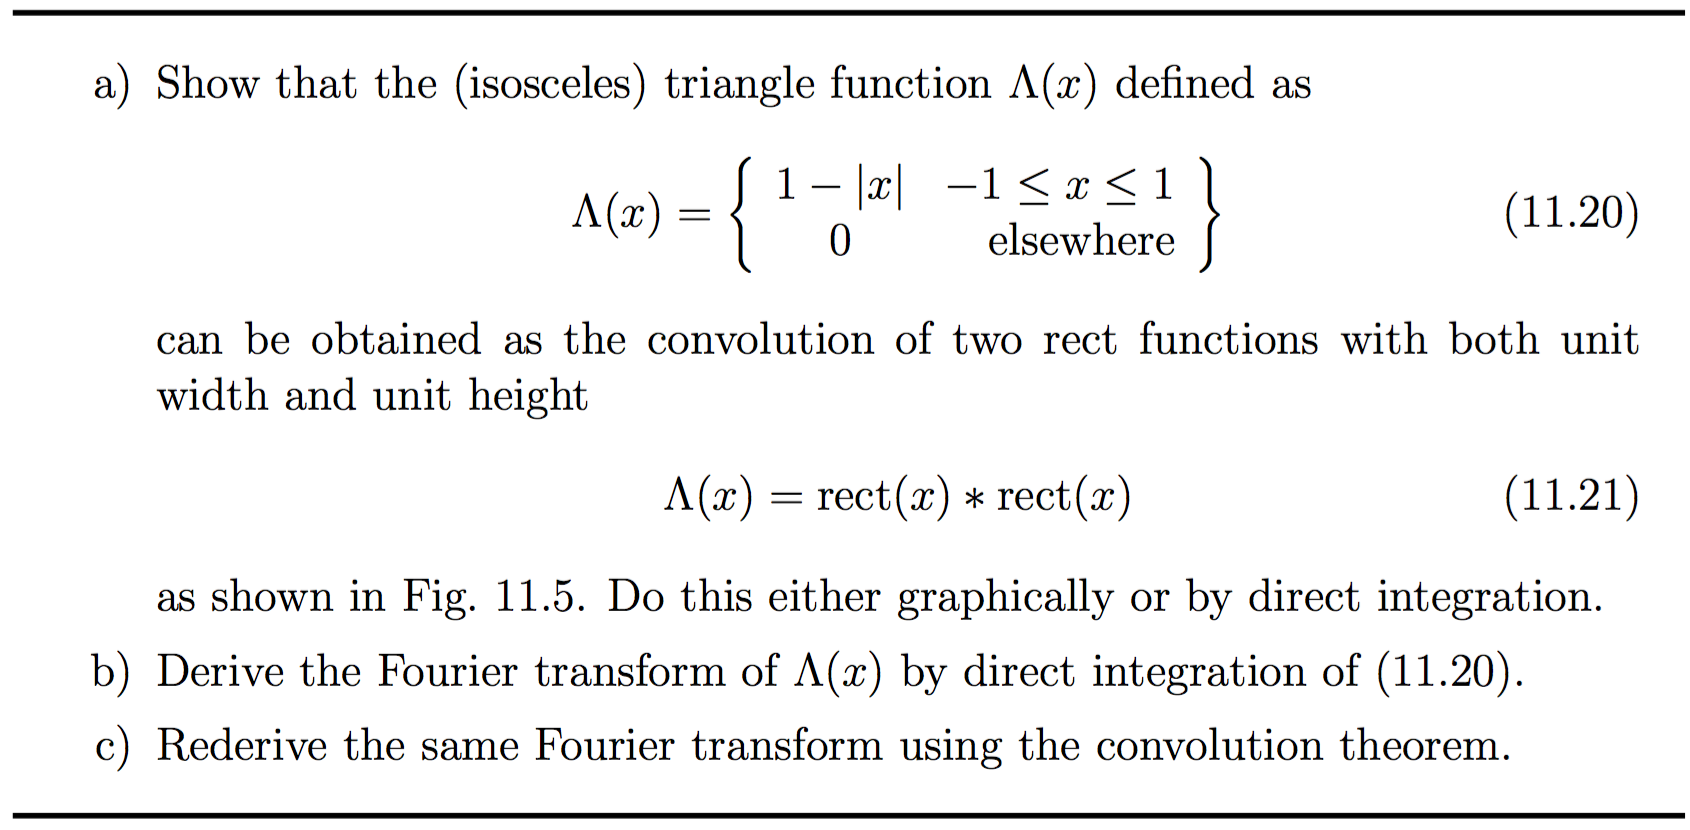
\includegraphics[width=1\textwidth,keepaspectratio]{prbl116}
    \label{fig:prbl116}
\end{figure}

\textit{Remember:}
\begin{itemize}
	\item 
\end{itemize}

\textit{Definitions:}


\textit{Proof.}

\clearpage
%%%%%%%%%%%%%%%%%%%%%%%%%%%%%%


%%%%%%%%%%%%%%%%%%%%%%%%%%%%%%
\Large{Problem 11.7}
\begin{figure}[H]
    \centering
    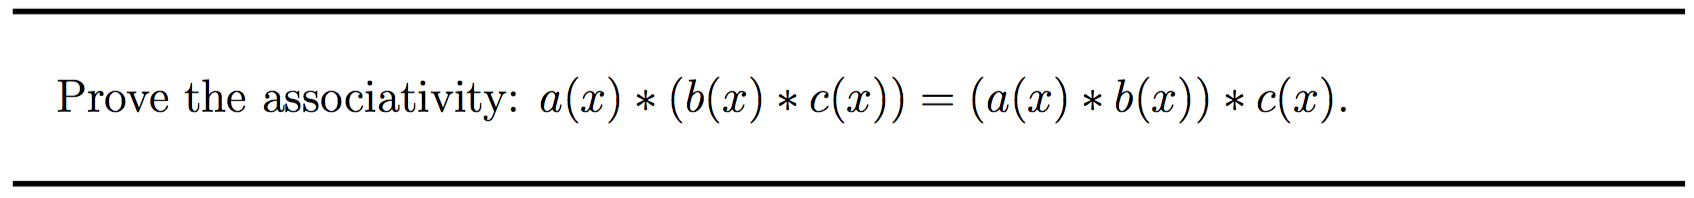
\includegraphics[width=1\textwidth,keepaspectratio]{prbl117}
    \label{fig:prbl117}
\end{figure}

\textit{Remember:}
\begin{itemize}
	\item 
\end{itemize}

\textit{Definitions:}


\textit{Proof.}

\clearpage
%%%%%%%%%%%%%%%%%%%%%%%%%%%%%%


%%%%%%%%%%%%%%%%%%%%%%%%%%%%%%
\Large{Problem 11.8}
\begin{figure}[H]
    \centering
    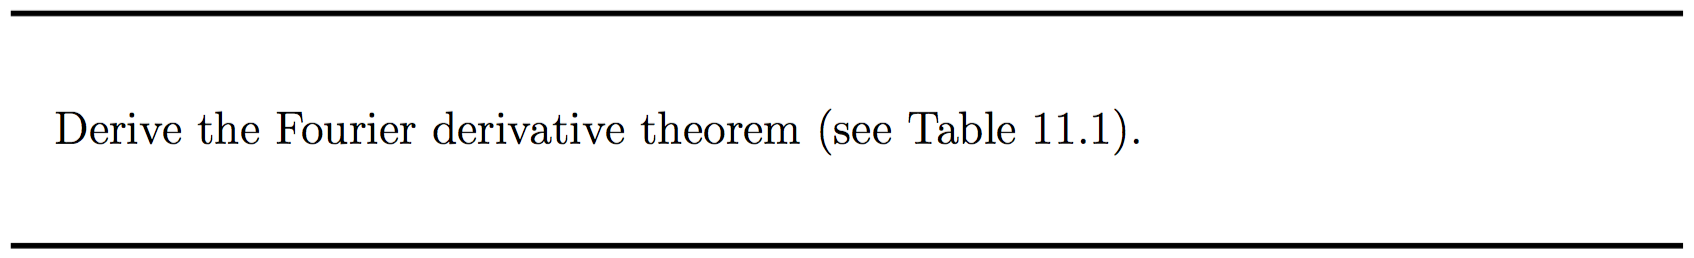
\includegraphics[width=1\textwidth,keepaspectratio]{prbl118}
    \label{fig:prbl118}
\end{figure}

\textit{Remember:}
\begin{itemize}
	\item 
\end{itemize}

\textit{Definitions:}


\textit{Proof.}

\clearpage
%%%%%%%%%%%%%%%%%%%%%%%%%%%%%%



%%%%%%%%%%%%%%%%%%%%%%%%%%%%%%
\Large{Problem 11.9}
\begin{figure}[H]
    \centering
    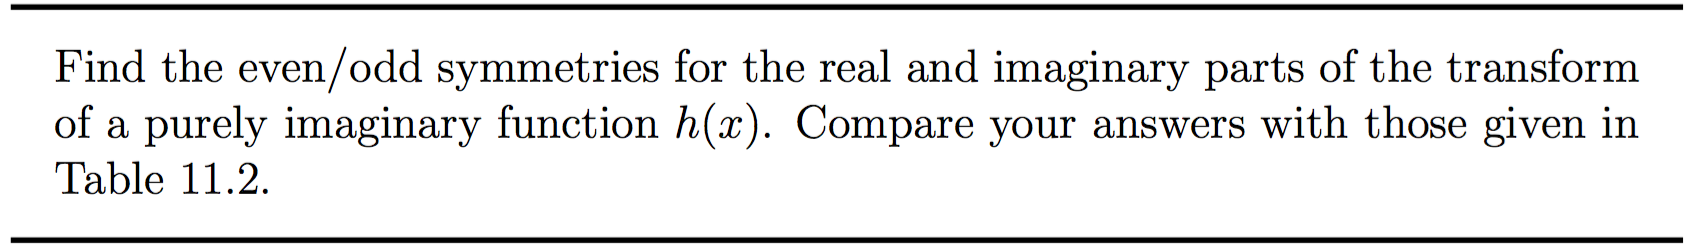
\includegraphics[width=1\textwidth,keepaspectratio]{prbl119}
    \label{fig:prbl119}
\end{figure}

\textit{Remember:}
\begin{itemize}
	\item 
\end{itemize}

\textit{Definitions:}


\textit{Proof.}

\clearpage
%%%%%%%%%%%%%%%%%%%%%%%%%%%%%%


%%%%%%%%%%%%%%%%%%%%%%%%%%%%%%
\Large{Problem 11.10}
\begin{figure}[H]
    \centering
    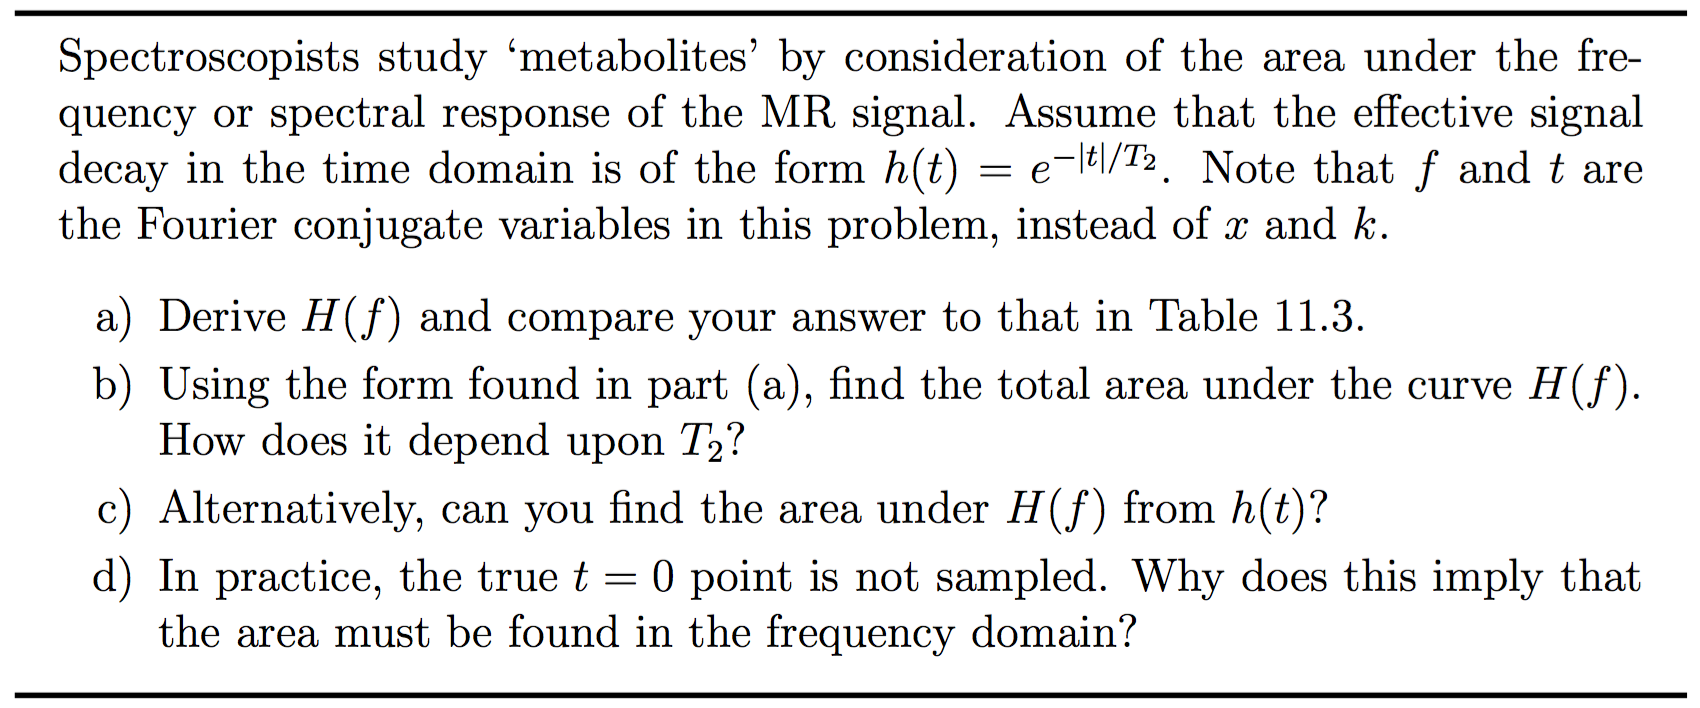
\includegraphics[width=1\textwidth,keepaspectratio]{prbl1110}
    \label{fig:prbl1110}
\end{figure}

\textit{Remember:}
\begin{itemize}
	\item 
\end{itemize}

\textit{Definitions:}


\textit{Proof.}

\clearpage
%%%%%%%%%%%%%%%%%%%%%%%%%%%%%%


%%%%%%%%%%%%%%%%%%%%%%%%%%%%%%
\Large{Problem 11.11}
\begin{figure}[H]
    \centering
    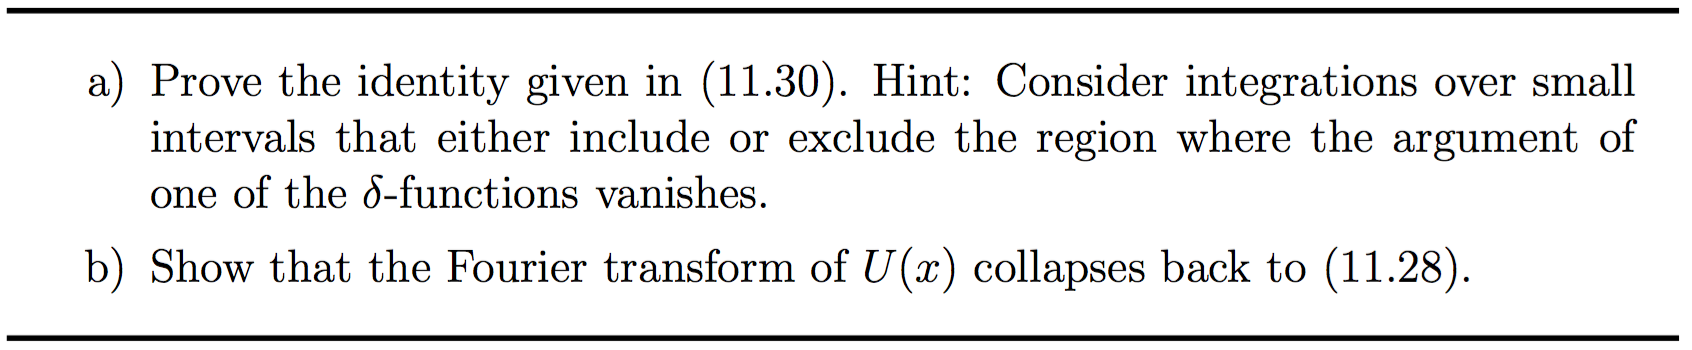
\includegraphics[width=1\textwidth,keepaspectratio]{prbl1111}
    \label{fig:prbl1111}
\end{figure}

\textit{Remember:}
\begin{itemize}
	\item 
\end{itemize}

\textit{Definitions:}


\textit{Proof.}

\clearpage
%%%%%%%%%%%%%%%%%%%%%%%%%%%%%%


%%%%%%%%%%%%%%%%%%%%%%%%%%%%%%
\Large{Problem 11.12}
\begin{figure}[H]
    \centering
    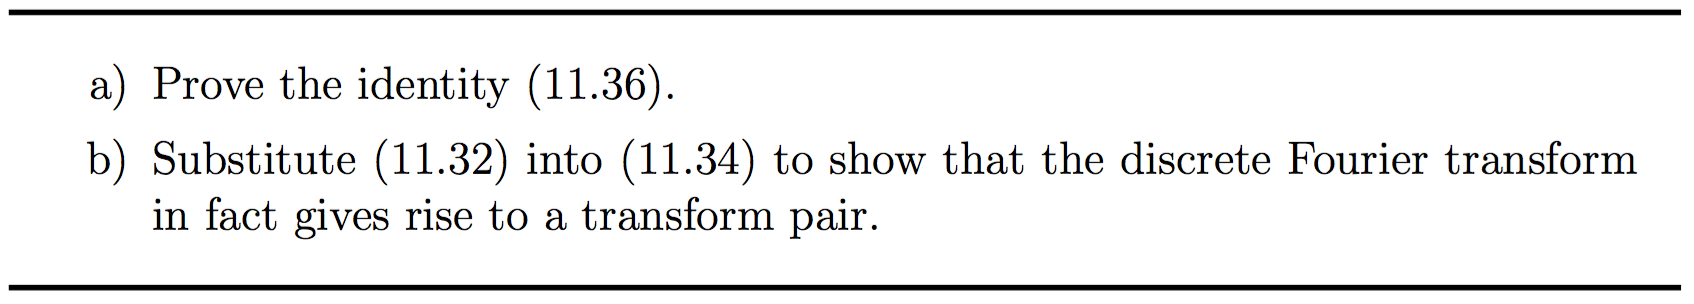
\includegraphics[width=1\textwidth,keepaspectratio]{prbl1112}
    \label{fig:prbl1112}
\end{figure}

\textit{Remember:}
\begin{itemize}
	\item 
\end{itemize}

\textit{Definitions:}


\textit{Proof.}

\clearpage
%%%%%%%%%%%%%%%%%%%%%%%%%%%%%%



%%%%%%%%%%%%%%%%%%%%%%%%%%%%%%
\Large{Problem 11.13}
\begin{figure}[H]
    \centering
    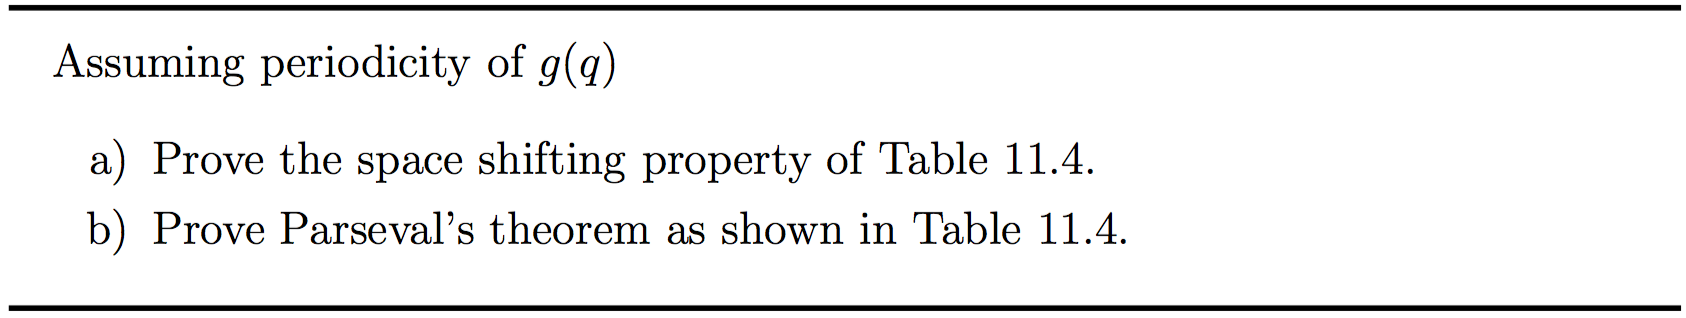
\includegraphics[width=1\textwidth,keepaspectratio]{prbl1113}
    \label{fig:prbl1113}
\end{figure}

\textit{Remember:}
\begin{itemize}
	\item 
\end{itemize}

\textit{Definitions:}


\textit{Proof.}

\clearpage
%%%%%%%%%%%%%%%%%%%%%%%%%%%%%%



%%%%%%%%%%%%%%%%%%%%%%%%%%%%%%
\Large{Problem 11.14}
\begin{figure}[H]
    \centering
    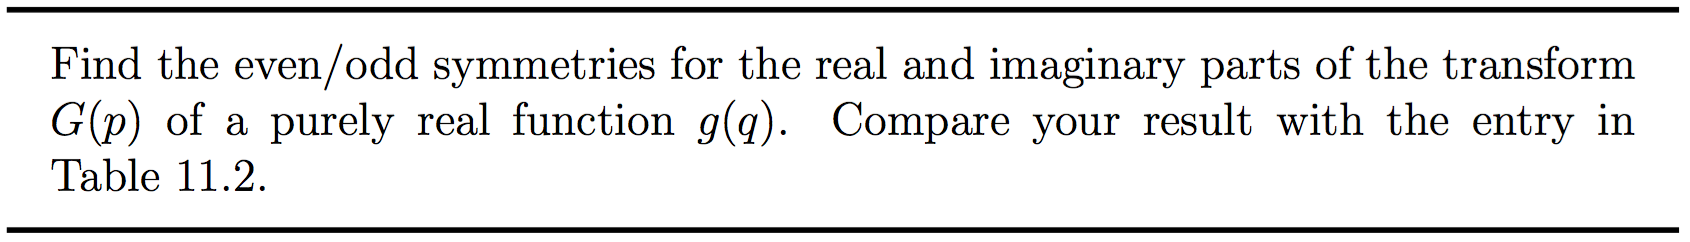
\includegraphics[width=1\textwidth,keepaspectratio]{prbl1114}
    \label{fig:prbl1114}
\end{figure}

\textit{Remember:}
\begin{itemize}
	\item 
\end{itemize}

\textit{Definitions:}


\textit{Proof.}

\clearpage
%%%%%%%%%%%%%%%%%%%%%%%%%%%%%%












